\newpage
~
\newpage
\chapter{Estado del Arte}
% Qué se ha hecho hasta ahora en este campo, qué tecnologías se han utilizado, qué problemas se han encontrado, qué soluciones se han propuesto.

En este capítulo se presenta un análisis del estado del arte en el ámbito de las bibliotecas de archivos multimedia de código abierto (\acrfull{foss}).
Se examinan las principales soluciones disponibles, sus características técnicas, fortalezas y limitaciones, así como las tendencias actuales en el sector.
Dado que uno de los objetivos del proyecto es desarrollar un producto que sea de código abierto, la comparación se centra en soluciones FOSS que ya están en el mercado y que han sido ampliamente adoptadas por la comunidad, lo cual nos va a permitir desarrollar una comparación mas extensa sobre cómo están organizados los proyectos para facilitar su mantenimiento y escalabilidad, así como las tecnologías que utilizan para ofrecer sus servicios.

Además, se realiza un estudio sobre las tecnologías que vamos a utilizar en el proyecto en comparación con las alternativas y las que ya se utilizan en los proyectos existentes que se analizan.

En el panorama actual de las bibliotecas de archivos multimedia de código abierto, existe una amplia variedad de soluciones que buscan ofrecer alternativas libres y gratuitas a los servicios propietarios como Google Photos o iCloud. Este análisis del estado del arte se centra en las tres soluciones de código abierto gratuitas más populares según el número de estrellas en GitHub: Immich, PhotoPrism y Ente.

% Fuentes:
% Google Photos: https://photos.google.com/
% Apple Photos: https://www.apple.com/ios/photos/
% Amazon Photos: https://www.amazon.com/photos
% Microsoft OneDrive Photos: https://www.microsoft.com/en-us/microsoft-365/onedrive/online-cloud-storage
\section{Sistemas de almacenamiento y compartición de contenidos multimedia}

Un sistema de almacenamiento y compartición de contenidos multimedia puede entenderse como una plataforma que permite a los usuarios guardar, organizar y acceder a recursos como fotografías, vídeos o grabaciones de audio desde diferentes dispositivos y ubicaciones. Este tipo de sistemas han surgido en gran medida como alternativa a las soluciones comerciales de almacenamiento en la nube, ofreciendo en muchos casos un mayor control sobre la privacidad y la gestión de los datos.

La primera característica esencial de este tipo de soluciones es el soporte multiusuario y la concurrencia, que posibilitan que varias personas interactúen con el sistema de manera simultánea sin comprometer la coherencia de la información. Esta propiedad se complementa con la sincronización automática, mediante la cual los contenidos capturados en un dispositivo, como puede ser un teléfono móvil, se transfieren y actualizan de manera transparente en el servidor, garantizando que los usuarios dispongan siempre de la versión más reciente de sus archivos.

Otra dimensión relevante es la accesibilidad multiplataforma: un mismo repositorio de información debe poder consultarse desde ordenadores, tablets o dispositivos móviles, ya sea mediante aplicaciones específicas o a través de interfaces web adaptadas. A medida que el volumen de datos crece, la escalabilidad se convierte en un requisito imprescindible, ya que el sistema debe mantener un rendimiento adecuado incluso en contextos con gran número de usuarios o con repositorios de gran tamaño.

Además de estas capacidades técnicas, estos sistemas suelen incluir mecanismos de organización basados en metadatos, como fechas, ubicaciones geográficas o etiquetas, lo que permite una gestión más eficiente y flexible de grandes colecciones de contenido. La privacidad y la seguridad representan otro pilar fundamental: la autenticación, la autorización y, en muchos casos, el cifrado, son necesarios para garantizar que los datos personales permanezcan protegidos frente a accesos no autorizados. 

Del mismo modo, la compartición de contenidos constituye un aspecto central. La posibilidad de compartir álbumes, carpetas o ficheros con otros usuarios, mediante enlaces públicos o controles de acceso más detallados, amplía las capacidades colaborativas del sistema. Finalmente, muchas de estas plataformas integran funciones de copia de seguridad y recuperación que aseguran la resiliencia frente a fallos, evitando la pérdida de información crítica.

En conjunto, estas propiedades conforman el núcleo de lo que se entiende actualmente por un sistema de almacenamiento y compartición de contenidos multimedia. A partir de esta base conceptual, en las siguientes secciones se examinarán diversas soluciones consolidadas en este ámbito, con el fin de evaluar hasta qué punto responden a estos requisitos y qué innovaciones introducen respecto a los enfoques tradicionales.

\section{Soluciones propietarias relevantes}

En el ámbito de la gestión y almacenamiento de fotografías, las soluciones propietarias han marcado el estándar en cuanto a experiencia de usuario, integración de servicios y capacidades avanzadas de inteligencia artificial. Entre las plataformas más destacadas se encuentran Google Photos, Apple Photos, Amazon Photos y Microsoft OneDrive Photos, cada una con un enfoque particular y funcionalidades diferenciadoras.

Google Photos sobresale por su motor de búsqueda semántica basado en inteligencia artificial, que permite localizar imágenes mediante descripciones textuales, reconocimiento automático de objetos, lugares y personas, así como la agrupación inteligente de rostros. Además, ofrece funciones como la creación automática de álbumes, recuerdos personalizados, sugerencias de edición y generación de vídeos y animaciones a partir de colecciones de fotos. La integración con Google Assistant permite búsquedas por voz y automatización de tareas relacionadas con la gestión de imágenes.

Apple Photos, por su parte, se integra de forma nativa en el ecosistema de dispositivos Apple, ofreciendo sincronización automática y segura a través de iCloud. Destaca por sus potentes herramientas de edición no destructiva, la organización automática mediante “Memories” y “People”, y la privacidad reforzada mediante el procesamiento local de datos sensibles, como el reconocimiento facial. La integración con Siri permite búsquedas contextuales y sugerencias inteligentes.

Amazon Photos ofrece almacenamiento ilimitado de fotografías en alta resolución para suscriptores de Amazon Prime, así como detección automática de duplicados y organización por personas, lugares y objetos. Su enfoque está orientado a la simplicidad y la capacidad de compartir álbumes de forma privada o pública, además de la integración con dispositivos Amazon Echo Show para visualización mediante comandos de voz.

Microsoft OneDrive Photos integra la gestión de imágenes con el resto de servicios de productividad de Microsoft 365, facilitando la colaboración y el acceso multiplataforma. Incluye funciones de etiquetado automático, búsqueda por contenido visual y organización cronológica, así como integración con herramientas de edición en línea y sincronización con dispositivos Windows y móviles.

Entre las características avanzadas que suelen estar más desarrolladas en estas soluciones propietarias, y que pueden servir de inspiración para el desarrollo de alternativas open-source, destacan:
\begin{itemize}
    \item \textbf{Búsqueda semántica avanzada}: Localización de imágenes mediante descripciones naturales, reconocimiento de escenas, objetos y personas.
    \item \textbf{Agrupación y etiquetado inteligente}: Detección y agrupación automática de rostros, lugares y eventos.
    \item \textbf{Generación automática de recuerdos y contenido}: Creación de álbumes, vídeos y animaciones personalizadas a partir de colecciones de fotos.
    \item \textbf{Integración con asistentes virtuales}: Búsqueda y gestión de imágenes mediante comandos de voz.
    \item \textbf{Sincronización y acceso multiplataforma}: Integración transparente con diferentes dispositivos y sistemas operativos.
    \item \textbf{Herramientas avanzadas de edición}: Edición no destructiva, sugerencias automáticas y filtros inteligentes.
    \item \textbf{Privacidad y control de datos}: Procesamiento local de información sensible y opciones avanzadas de control de acceso.
\end{itemize}

Si bien algunas de estas funcionalidades comienzan a estar presentes en proyectos de código abierto, la madurez, precisión y facilidad de uso de las implementaciones propietarias sigue siendo, en muchos casos, superior debido a la inversión en inteligencia artificial, recursos computacionales y la integración profunda con sus respectivos ecosistemas. La incorporación de estas capacidades en soluciones FOSS representa un reto y una oportunidad para cerrar la brecha funcional existente.

\section{Panorama general de soluciones FOSS}

El ecosistema de soluciones FOSS ha experimentado un crecimiento significativo en los últimos años, impulsado por las crecientes preocupaciones sobre la privacidad de los datos y la dependencia de servicios en la nube propietarios. Según el análisis comparativo realizado por Meichthys \parencite{meichthys2024}, existen más de 16 proyectos activos que ofrecen diferentes enfoques y características.

Las soluciones analizadas se pueden clasificar en tres categorías principales:
\begin{itemize}
    \item \textbf{Soluciones escalables}: Enfocadas en escalabilidad y características avanzadas
    \item \textbf{Soluciones centradas en privacidad}: Priorizan la seguridad y el cifrado
    \item \textbf{Soluciones ligeras}: Optimizadas para recursos limitados
\end{itemize}

% --- NUEVA ORGANIZACIÓN: ANÁLISIS INDIVIDUAL DE CADA SOLUCIÓN ---

\section{Immich}

(\cite{immich-documentation}) Immich es una solución de gestión de fotos de código abierto orientada a usuarios que buscan una alternativa privada y autoalojada a servicios comerciales como Google Photos. Su desarrollo comenzó en 2022 y ha experimentado un rápido crecimiento gracias a una comunidad activa y a la adopción de tecnologías modernas.

\textbf{Propósito y público objetivo:} Immich está diseñado para usuarios particulares, familias y pequeños equipos que desean mantener el control sobre sus fotos y vídeos, evitando la dependencia de servicios en la nube de terceros. Es especialmente atractivo para entusiastas de la tecnología y defensores de la privacidad.

\textbf{Historia y contexto:} El proyecto nació como respuesta a la falta de alternativas libres y modernas a los grandes servicios comerciales, con un enfoque en la experiencia de usuario y la facilidad de despliegue.

\textbf{Modelo de desarrollo:} Immich es mantenido principalmente por una comunidad de desarrolladores en GitHub, con contribuciones frecuentes y una hoja de ruta pública.

\textbf{Características funcionales:}
\begin{itemize}
    \item \textbf{Aplicaciones móviles y web}: Apps nativas para Android e iOS, y una interfaz web moderna y responsiva.
    \item \textbf{Copia de seguridad automática}: Respaldo automático de fotos y vídeos desde dispositivos móviles.
    \item \textbf{Soporte multiplataforma}: Disponible en web y dispositivos móviles, con sincronización automática.
    \item \textbf{Reconocimiento facial y de objetos}: Identificación automática de personas y elementos en las fotos.
    \item \textbf{Búsqueda avanzada}: Permite buscar por etiquetas, ubicaciones, fechas y otros metadatos.
    \item \textbf{Vista de carpetas}: Navegación por la estructura de carpetas original.
    \item \textbf{Soporte de Chromecast}: Permite enviar fotos y vídeos a dispositivos Chromecast.
    \item \textbf{Transcodificación y aceleración hardware}: Soporte para transcodificación de vídeo y aceleración por hardware.
    \item \textbf{Librerías externas}: Indexación de archivos existentes en el disco sin necesidad de moverlos.
    \item \textbf{Gestión de usuarios y roles}: Configuración de cuentas, ajustes y permisos.
    \item \textbf{Etiquetas y álbumes}: Organización mediante etiquetas y álbumes personalizados.
    \item \textbf{Compartición}: Compartir álbumes y fotos mediante enlaces o con otros usuarios.
    \item \textbf{Soporte de XMP sidecars}: Lectura y escritura de metadatos en archivos sidecar XMP.
    \item \textbf{CLI y monitorización}: Herramienta de línea de comandos y panel de monitorización.
    \item \textbf{Soporte de formatos}: Compatibilidad con JPEG, PNG, HEIC, RAW (parcial), vídeos y Live Photos.
    \item \textbf{Traducción}: Disponible en varios idiomas, incluyendo español.
\end{itemize}

\textbf{Comunidad y ecosistema:}
\begin{itemize}
    \item \textbf{Comunidad activa}: Foros, Discord y GitHub con alta participación.
    \item \textbf{Documentación}: Completa y en constante actualización.
    \item \textbf{Extensibilidad}: API pública y soporte para integraciones futuras.
\end{itemize}

\textbf{Seguridad y privacidad:}
\begin{itemize}
    \item \textbf{Gestión de datos personales}: Los datos permanecen en el servidor del usuario, sin envíos a terceros.
    \item \textbf{Cifrado}: Actualmente no implementa cifrado de extremo a extremo, pero sí buenas prácticas de seguridad en el almacenamiento y acceso.
    \item \textbf{Actualizaciones}: Lanzamientos frecuentes y respuesta rápida a vulnerabilidades.
\end{itemize}

\textbf{Casos de uso y ejemplos reales:}
\begin{itemize}
    \item Utilizado por usuarios domésticos y pequeñas organizaciones para gestionar colecciones fotográficas privadas.
    \item Referencias y testimonios positivos en foros de autoalojamiento y privacidad.
\end{itemize}

\textbf{Limitaciones actuales:}
\begin{itemize}
    \item Alto consumo de recursos debido a Node.js.
    \item API en constante evolución (su última versión aún no se considera estable).
    \item Algunas funciones avanzadas (como la edición colaborativa) están en desarrollo.
    \item La integración con otros servicios y dispositivos aún es limitada en comparación con soluciones comerciales.
\end{itemize}

\textbf{Importación de archivos existentes}

(\cite{immich-documentation}, \href{https://immich.app/docs/features/libraries/}{Librerías externas}) Immich permite importar archivos multimedia ya existentes en el disco mediante el uso de \textit{external libraries}. Estas bibliotecas externas rastrean los archivos almacenados fuera de Immich y, al escanearlas, la aplicación indexa fotos y vídeos desde las rutas configuradas (import paths), mostrándolos en la línea de tiempo principal como cualquier otro recurso. Los archivos pueden organizarse en varias bibliotecas, cada una con múltiples rutas de importación, y se pueden definir patrones de exclusión para omitir ciertos archivos o carpetas (por ejemplo, RAW). Si un archivo se elimina del disco, Immich lo mueve a la papelera tras un nuevo escaneo; si se modifica fuera de Immich, es necesario volver a escanear para reflejar los cambios. La importación requiere que las rutas sean accesibles desde el contenedor Docker de Immich, por lo que es necesario montar los volúmenes correspondientes. Además, existe una función experimental de vigilancia automática del sistema de archivos para importar nuevos archivos sin necesidad de escanear manualmente. Es importante tener en cuenta que los metadatos añadidos desde Immich no se escriben en los archivos originales, y que mover archivos fuera de las rutas de importación puede hacer que se pierdan los metadatos asociados en Immich.

\textbf{Requisitos de Hardware}

(\cite{immich-documentation}, \href{https://immich.app/docs/install/requirements}{Apartado de requerimientos}) Immich presenta los siguientes requisitos de hardware para su instalación y funcionamiento óptimo:

\begin{itemize}
    \item Recomendado sistema operativo Linux o variante de UNIX para una mejor compatibilidad con Docker.
    \item Procesador con al menos 2 núcleos, recomendado 4 o más.
    \item Mínimo de 4 GB de RAM, recomendado 6 GB o más.
    \item Recomendado sistema de almacenamiento UNIX (EXT4, ZFS, APFS, etc.) que ofrezca soporte para permisos y propiedad de usuarios/grupos.
    \item Se recomienda tener la base de datos en un dispositivo SSD y con una conexión rápida y estable, puesto que los archivos de PostgreSQL pueden crecer rápidamente.
\end{itemize}

\textbf{Arquitectura}

(\cite{immich-documentation}, \href{https://immich.app/docs/developer/architecture/}{Apartado de arquitectura}) Immich utiliza una arquitectura cliente-servidor. Además, implementa una separación de responsabilidades haciendo uso de una arquitectura hexagonal un tanto relajado, puesto que no la siguen al pie de la letra si no que buscan separar la lógica de negocio de la lógica de infraestructura, tanto para el cliente como el servidor:

\begin{figure}[H]
  \centering
  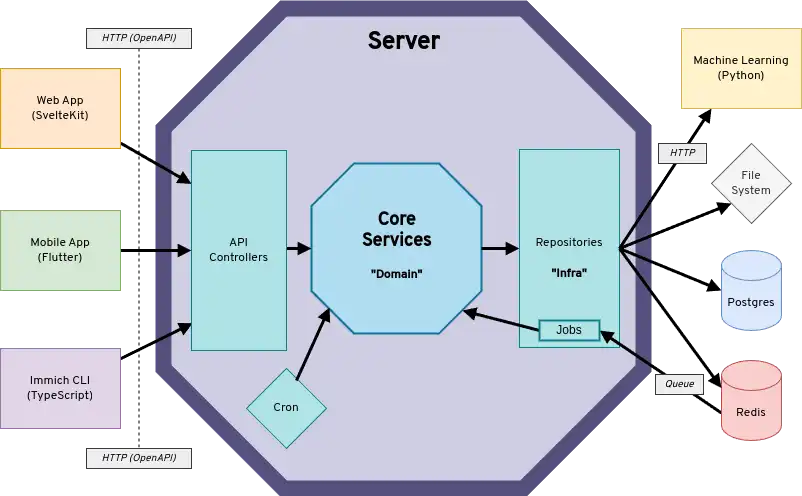
\includegraphics[width=0.8\textwidth]{assets/immich-architecture.png}
  \caption{Arquitectura de Immich (\cite{immich-documentation}, \href{https://immich.app/docs/developer/architecture/}{Apartado de arquitectura})}
  \label{fig:immich-architecture}
\end{figure}


\begin{figure}[H]
  \centering
  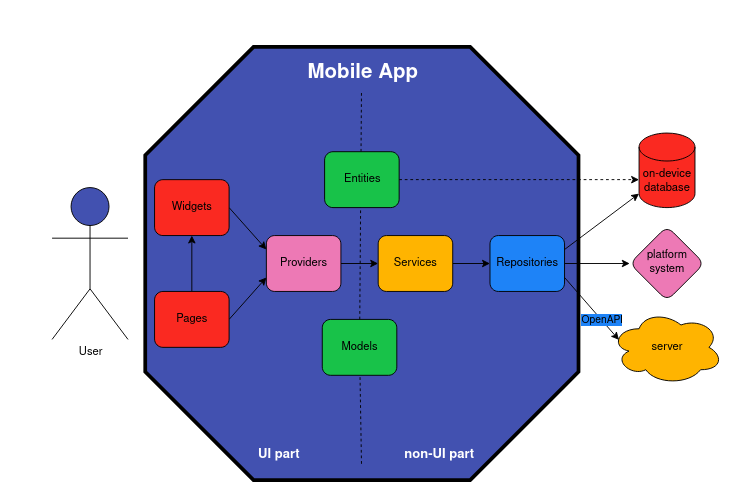
\includegraphics[width=0.8\textwidth]{assets/immich-architecture-client.png}
  \caption{Arquitectura del cliente de Immich (\cite{immich-documentation}, \href{https://immich.app/docs/developer/architecture/}{Apartado de arquitectura})}
  \label{fig:immich-architecture-client}
\end{figure}

Aunque en teoría utilizan esta arquitectura, en la práctica se observa que no siempre se sigue al pie de la letra.

\textbf{Escalabilidad}

(\cite{immich-documentation}, \href{https://immich.app/docs/guides/scaling-immich/}{Apartado de escalabilidad}) Immich ha sido desarrollado siguiendo prácticas modernas de despliegue, permitiendo la ejecución de múltiples instancias del backend de manera paralela. Para implementar una escalabilidad horizontal efectiva, es imprescindible que todas las instancias estén conectadas a una infraestructura compartida, lo que implica el acceso común a la base de datos Postgres, al sistema de colas Redis y al almacenamiento de archivos.

\begin{itemize}
    \item \textbf{Escalabilidad vertical:} El rendimiento del sistema puede incrementarse mediante la ampliación de los recursos de hardware en una única máquina. Immich está optimizado para aprovechar múltiples tareas en segundo plano, cuyo número puede ser ajustado desde el panel de administración.
    \item \textbf{Escalabilidad horizontal:} Es posible desplegar varias instancias de Immich en diferentes máquinas o contenedores, lo cual resulta especialmente ventajoso en entornos orquestados como Kubernetes o en escenarios donde se desea aprovechar recursos distribuidos (por ejemplo, usar un PC potente para tareas de transcodificación). Todas las instancias deben compartir la misma base de datos, Redis y almacenamiento de archivos. La configuración concreta depende del entorno y puede requerir conocimientos adicionales (NFS, túneles de red, etc.).
    \item \textbf{Gestión de workers:} Cada contenedor de Immich ejecuta varios workers internos. Si el objetivo del escalado es únicamente aumentar la capacidad de procesamiento en segundo plano, se puede deshabilitar el worker de API en instancias adicionales para optimizar recursos.
    \item \textbf{Escalado hacia abajo:} Immich permite reducir el número de instancias sin riesgo de pérdida de información, ya que todo el estado se almacena en Postgres, Redis y el sistema de archivos. Las tareas pendientes quedarán en espera hasta que haya workers disponibles.
\end{itemize}

Cabe destacar que, en escenarios con una sola máquina, el escalado horizontal no suele aportar beneficios adicionales, ya que cada contenedor puede gestionar múltiples tareas concurrentemente.

\textbf{Monetización}

Immich es completamente gratuito y open source, sin funciones premium o de pago. Su financiación proviene de donaciones y de la comunidad.

\textbf{Interoperabilidad}

Immich presenta las siguientes características de interoperabilidad:

\begin{itemize}
    \item \textbf{Integración con servicios externos:} Soporte para almacenamiento externo mediante protocolos como \gls{webdav} y \gls{s3}.
    \item \textbf{Soporte de estándares de metadatos:} Soporte parcial, centrado principalmente en EXIF.
    \item \textbf{Exportación e importación:} Permite la exportación e importación de fotos y metadatos, con algunas limitaciones.
    \item \textbf{Federación y APIs:} Ofrece APIs REST para integración con aplicaciones de terceros, con una API en evolución.
\end{itemize}

% --- FIN DE ANÁLISIS INDIVIDUAL DE Immich ---

\section{PhotoPrism}

(\cite{photoprism-documentation}) PhotoPrism es una de las soluciones FOSS más maduras y populares para la gestión de fotos, con una comunidad consolidada y un enfoque en la organización eficiente y el respeto a la privacidad.

\textbf{Propósito y público objetivo:} Orientado a usuarios que buscan una alternativa autoalojada, robusta y fácil de usar para organizar grandes colecciones de fotos, con especial atención a la preservación de metadatos y la integración con sistemas existentes.

\textbf{Historia y contexto:} Lanzado en 2017, PhotoPrism ha evolucionado para convertirse en una referencia dentro del software libre de gestión fotográfica, con un desarrollo sostenido y una base de usuarios creciente.

\textbf{Modelo de desarrollo:} Proyecto comunitario con liderazgo claro, financiado parcialmente por donaciones y patrocinios.

\textbf{Características funcionales:}
\begin{itemize}
    \item \textbf{Aplicación web progresiva (PWA)}: Experiencia similar a una app nativa en cualquier dispositivo, instalable en móviles y escritorio.
    \item \textbf{Soporte multiplataforma}: Funciona en Mac, Linux, Windows, Raspberry Pi, FreeBSD y NAS.
    \item \textbf{Búsqueda avanzada}: Filtros combinables por etiquetas, ubicación, resolución, color, calidad, etc.
    \item \textbf{Reconocimiento facial}: Detección y agrupación de rostros para identificar personas.
    \item \textbf{Mapas y lugares}: Visualización de fotos en mapas de alta resolución y enriquecimiento de metadatos de ubicación.
    \item \textbf{Compartición de álbumes}: Enlaces secretos con expiración opcional, sin necesidad de registro.
    \item \textbf{Soporte de formatos}: Indexación, visualización y conversión de imágenes, vídeos y RAW (JPEG, PNG, GIF, BMP, HEIF, HEIC, MP4, MOV, WebP, WebM, y amplia compatibilidad RAW).
    \item \textbf{Extracción avanzada de metadatos}: Soporte para Exif, XMP, Google Photos JSON y normalización de campos.
    \item \textbf{Detección de duplicados}: Identificación automática de archivos repetidos.
    \item \textbf{Sincronización y backup}: Integración con PhotoSync y clientes WebDAV para copia de seguridad y acceso remoto.
    \item \textbf{Privacidad}: 100\% autoalojado, sin compartir datos con terceros.
    \item \textbf{Etiquetas, álbumes y organización}: Clasificación flexible y apilado de fotos relacionadas.
    \item \textbf{Revisión y selección}: Herramientas para marcar, archivar, ocultar o revisar fotos.
    \item \textbf{Soporte de sidecars}: Uso de archivos sidecar para metadatos.
    \item \textbf{Temas claro/oscuro}: Interfaz adaptable.
\end{itemize}

\textbf{Comunidad y ecosistema:}
\begin{itemize}
    \item \textbf{Comunidad consolidada}: Foros, GitHub y canales de soporte activos.
    \item \textbf{Documentación}: Muy completa y detallada.
    \item \textbf{Extensibilidad}: API básica y soporte de sidecars.
\end{itemize}

\textbf{Seguridad y privacidad:}
\begin{itemize}
    \item \textbf{Gestión de datos personales}: Los datos permanecen bajo control del usuario.
    \item \textbf{Cifrado}: No implementa cifrado de extremo a extremo, pero permite despliegues seguros en redes privadas.
    \item \textbf{Actualizaciones}: Ciclo de lanzamientos estable y respuesta adecuada a incidencias.
\end{itemize}

\textbf{Casos de uso y ejemplos reales:}
\begin{itemize}
    \item Utilizado por fotógrafos (por su compatibilidad sencilla con tipos de imágenes RAW), familias y pequeñas empresas para organizar y buscar fotos de forma eficiente.
    \item Referencias en comunidades de software libre y autoalojamiento.
\end{itemize}

\textbf{Limitaciones actuales:}
\begin{itemize}
    \item Soporte limitado para múltiples usuarios (no orientado a uso multiusuario avanzado).
    \item Escalabilidad horizontal restringida.
    \item Aplicaciones móviles limitadas a PWA, sin apps nativas.
    \item No utiliza una estructura estandarizada para la organización, dificultando la contribución de terceros.
    \item No dispone de edición avanzada ni IA en el dispositivo.
\end{itemize}

\textbf{Importación de archivos existentes}

(\cite{photoprism-documentation}, \href{https://docs.photoprism.app/developer-guide/media/import/}{Importación de archivos}) PhotoPrism ofrece varias opciones para importar y gestionar archivos ya existentes en el disco. Es posible indexar directamente las carpetas originales, manteniendo la estructura y nombres de archivos, o utilizar la función de importación, que copia los archivos, elimina duplicados y los organiza automáticamente por año y mes. El modo de sólo lectura permite usar PhotoPrism como galería sin modificar los archivos originales. Además, se pueden subir archivos mediante WebDAV o la función de subida web, que los coloca en un directorio temporal antes de importarlos a la carpeta de originales. Tras la importación o indexación, PhotoPrism genera miniaturas y permite organizar, buscar y clasificar las fotos sin alterar los archivos fuente, salvo que se utilicen funciones avanzadas de importación.

\textbf{Requisitos de Hardware}

(\cite{photoprism-documentation}, \href{https://www.photoprism.app/plus/kb/requirements}{Apartado de requerimientos}) PhotoPrism recomienda los siguientes requisitos para su instalación y funcionamiento óptimo:

\begin{itemize}
    \item \textbf{Procesador:} Al menos 2 núcleos físicos, preferiblemente más para mejorar el rendimiento en tareas concurrentes e indexación de grandes colecciones.
    \item \textbf{Memoria RAM:} Mínimo 4 GB de memoria física; se recomienda igualar la cantidad de RAM al número de núcleos de CPU para un rendimiento óptimo, especialmente durante la indexación y procesamiento de archivos multimedia de gran tamaño.
    \item \textbf{Sistema operativo:} 64 bits, compatible con Docker Desktop (Windows 10+, macOS 11+), Podman (Red Hat, CentOS, Fedora, AlmaLinux, Rocky Linux) o Docker (Ubuntu, Debian y otras distribuciones Linux). Soporte multi-arquitectura para procesadores AMD, Intel y ARM64 (incluyendo Raspberry Pi 3/4 y Apple Silicon).
    \item \textbf{Almacenamiento:} Se recomienda el uso de SSD local para la base de datos y archivos de caché, lo que mejora significativamente el rendimiento en la indexación y acceso a miniaturas. El almacenamiento compartido en red o discos duros convencionales pueden utilizarse para la carpeta de originales, pero no para la base de datos ni la caché.
    \item \textbf{Espacio en disco:} Reservar aproximadamente un 50\% adicional del tamaño de los archivos originales para la carpeta de almacenamiento (miniaturas, caché y archivos generados). El uso real suele ser menor, dependiendo de la configuración y los tipos de archivo.
    \item \textbf{Swap:} Al menos 4 GB de espacio de swap para evitar reinicios inesperados durante el procesamiento de archivos grandes.
\end{itemize}

\textbf{Bases de datos compatibles:}
\begin{itemize}
    \item Compatible con SQLite 3 (recomendado solo para bibliotecas pequeñas o entornos de prueba) y MariaDB 10.5.12+ (recomendado para producción y grandes volúmenes de datos). El soporte para MySQL 8 ha sido discontinuado.
\end{itemize}

\textbf{Navegadores compatibles:}
\begin{itemize}
    \item La interfaz web, desarrollada como PWA, es compatible con los principales navegadores modernos (Chrome, Chromium, Safari, Firefox, Edge) y puede instalarse en la pantalla de inicio de sistemas operativos y dispositivos móviles.
\end{itemize}

\textbf{Notas adicionales:}
\begin{itemize}
    \item La conversión de imágenes RAW y el uso de TensorFlow se deshabilitan automáticamente en sistemas con 1 GB o menos de memoria.
    \item El uso de hardware más potente (mayor número de núcleos y RAM) mejora notablemente el rendimiento, especialmente en escenarios con múltiples usuarios concurrentes o grandes volúmenes de archivos.
    \item No se recomienda el uso de dispositivos NAS de gama baja ni almacenamiento no fiable (USB, SD, carpetas de red) para la base de datos.
\end{itemize}

\textbf{Arquitectura}

(\cite{photoprism-documentation}, \href{https://www.photoprism.app/kb/architecture}{Apartado de arquitectura}) PhotoPrism utiliza una arquitectura monolítica basada en contenedores Docker, lo que permite una fácil implementación y escalabilidad. La aplicación se compone de varios componentes principales:

\begin{figure}[h]
  \centering
  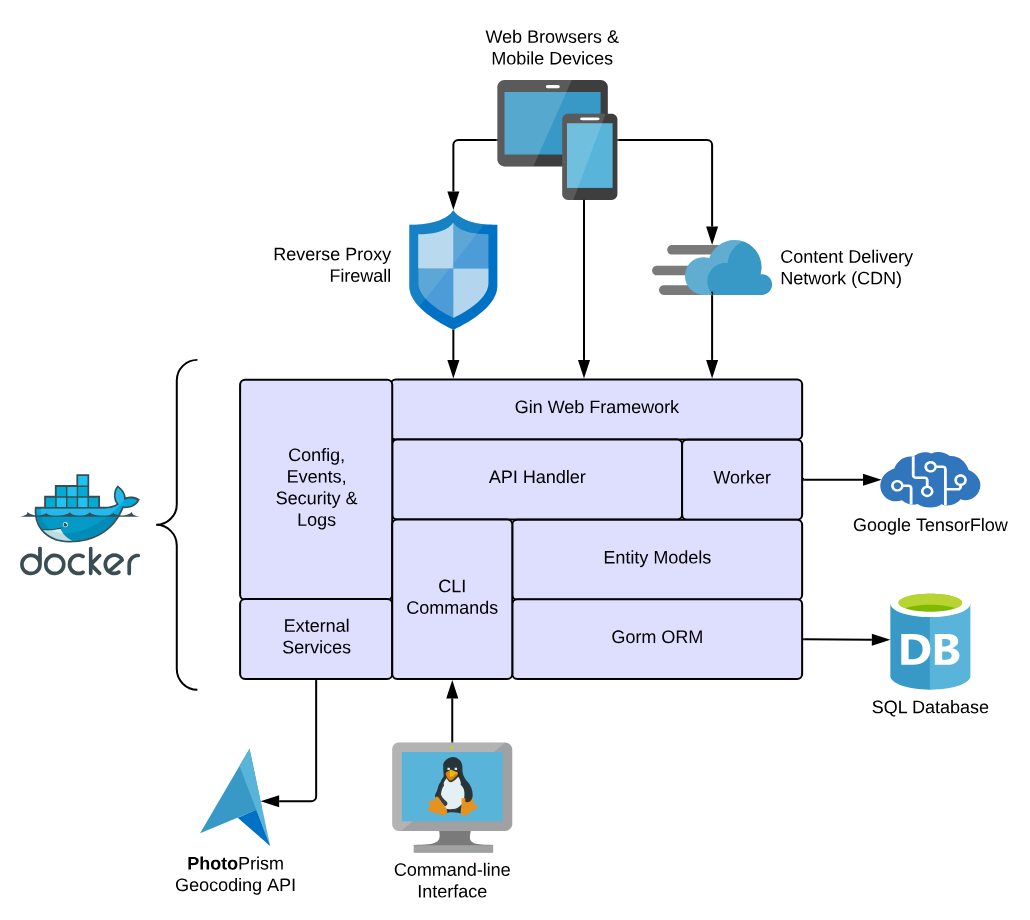
\includegraphics[width=0.8\textwidth]{assets/photoprism-modules.png}
  \caption{Arquitectura de monolito de PhotoPrism (\cite{photoprism-documentation}, \href{https://www.photoprism.app/kb/architecture}{Apartado de arquitectura})}
  \label{fig:photoprism-modules}
\end{figure}

Como podemos ver, aunque siguen una arquitectura monolítica, la aplicación está dividida en varios módulos cada uno con su responsabilidad
\textbf{Escalabilidad}

PhotoPrism está diseñado principalmente para maximizar el uso eficiente de los recursos disponibles, ya que la mayoría de sus usuarios lo ejecutan en dispositivos NAS domésticos o en pequeñas instancias de servidores en la nube. Por ello, tanto la documentación pública como el desarrollo del proyecto se centran en estos escenarios de uso.

\begin{itemize}
    \item \textbf{Escalabilidad vertical:} La edición Community Edition, disponible libremente, puede gestionar millones de archivos siempre que el servidor cumpla los requisitos recomendados. El rendimiento y la capacidad de la aplicación aumentan al mejorar los recursos de hardware (CPU, RAM, almacenamiento rápido), lo que permite manejar grandes volúmenes de datos y usuarios concurrentes en un único servidor.
    \item \textbf{Escalabilidad horizontal:} La arquitectura actual y el conjunto de funcionalidades no están orientados a la alta disponibilidad ni al escalado horizontal en la nube. Para escenarios empresariales que requieran alta disponibilidad o escalabilidad horizontal, sería necesario rediseñar la arquitectura, por ejemplo, dividiendo el backend en microservicios escalables de forma independiente y utilizando sistemas de almacenamiento distintos al sistema de archivos tradicional para la indexación.
\end{itemize}

En caso de requerimientos empresariales específicos de escalabilidad o disponibilidad, los desarrolladores de PhotoPrism ofrecen asesoramiento personalizado para evaluar la viabilidad y las opciones de implementación.

\textbf{Monetización}

PhotoPrism sigue un modelo freemium, donde algunas características avanzadas requieren suscripción. Existen membresías Plus y Pro disponibles.

\textbf{Interoperabilidad}

PhotoPrism presenta las siguientes características de interoperabilidad:

\begin{itemize}
    \item \textbf{Integración con servicios externos:} Soporte para almacenamiento externo mediante protocolos como \gls{webdav} y \gls{s3}.
    \item \textbf{Soporte de estándares de metadatos:} Soporte completo de estándares como EXIF, \acrshort{iptc} y \acrshort{xmp}.
    \item \textbf{Exportación e importación:} Facilita la migración mediante herramientas específicas y documentación detallada.
    \item \textbf{Federación y APIs:} Ofrece una API más estable para integración con aplicaciones de terceros.
\end{itemize}

% --- FIN DE ANÁLISIS INDIVIDUAL DE PhotoPrism ---

\section{Ente}

Ente destaca por su enfoque radical en la privacidad y la seguridad, ofreciendo cifrado de extremo a extremo y una experiencia multiplataforma coherente gracias a Flutter. Aunque su principal vía de uso es el servicio gestionado en la nube, Ente también soporta el autoalojamiento (\textit{self-hosting}), permitiendo a los usuarios desplegar su propio servidor siguiendo la documentación oficial\footnote{\url{https://help.ente.io/self-hosting/}}. Sin embargo, el autoalojamiento no es el foco principal del proyecto y la documentación, soporte y comunidad están más orientados al uso gestionado que a la personalización o despliegue avanzado por parte de terceros.

\textbf{Propósito y público objetivo:} Dirigido a usuarios que priorizan la privacidad y la seguridad de sus fotos, como periodistas, activistas o cualquier persona preocupada por la confidencialidad de sus datos. El modelo de negocio está basado en planes de suscripción y almacenamiento gestionado, aunque se ofrece la opción de autoalojamiento para usuarios avanzados.

\textbf{Historia y contexto:} Proyecto joven pero con rápido crecimiento, impulsado por la demanda de soluciones seguras y privadas en el ámbito de la gestión fotográfica. Ente ha puesto especial énfasis en la transparencia de su arquitectura y en la auditoría de su código, y aunque el autoalojamiento es posible y el código es abierto, la experiencia y el soporte están más orientados al servicio gestionado.

\textbf{Modelo de desarrollo:} Comunidad activa y transparente, con desarrollo abierto y enfoque en la seguridad, pero con la mayor parte de los esfuerzos centrados en el servicio gestionado.

\textbf{Características funcionales:}
\begin{itemize}
    \item \textbf{Cifrado de extremo a extremo}: Todas las fotos y metadatos se almacenan cifrados, solo el usuario puede acceder a ellos.
    \item \textbf{Replicación en 3 ubicaciones}: Los datos cifrados se almacenan en tres nubes distintas y ubicaciones geográficas.
    \item \textbf{Aplicaciones multiplataforma}: Apps para Android, iOS, Linux, Mac, Windows y web, todas open source.
    \item \textbf{Subida automática en segundo plano}: Copia de seguridad automática y continua en todos los dispositivos.
    \item \textbf{Planes familiares}: Compartición de suscripción con hasta 5 miembros, cada uno con espacio privado.
    \item \textbf{Búsqueda avanzada}: IA en el dispositivo para reconocimiento facial y búsqueda por lenguaje natural.
    \item \textbf{Compartición de álbumes}: Compartición cifrada con otros usuarios o mediante enlaces protegidos y configurables.
    \item \textbf{Colaboración}: Permite que otros usuarios añadan fotos a tus álbumes, incluso mediante enlaces públicos.
    \item \textbf{Importación y exportación}: Importación sencilla desde otros proveedores y exportación incremental con un clic.
    \item \textbf{Memorias}: Historias automáticas para revivir recuerdos de años anteriores.
    \item \textbf{Fotos ocultas}: Elementos protegidos tras la pantalla de bloqueo.
    \item \textbf{Descripciones y etiquetas}: Añadir descripciones y etiquetas cifradas, con búsqueda por palabras clave.
    \item \textbf{Seguridad adicional}: Autenticación en dos factores y bloqueo de pantalla.
    \item \textbf{Liberación de espacio}: Elimina archivos del dispositivo que ya han sido respaldados.
    \item \textbf{Temas claro/oscuro}: Interfaz adaptable en móviles.
    \item \textbf{Soporte y comunidad}: Soporte humano y comunidad activa.
\end{itemize}

\textbf{Comunidad y ecosistema:}
\begin{itemize}
    \item \textbf{Comunidad activa}: Desarrollo abierto y escucha activa de sugerencias.
    \item \textbf{Soporte humano}: Atención personalizada por correo.
    \item \textbf{Hoja de ruta pública}: Mejoras continuas y transparencia.
\end{itemize}

\textbf{Seguridad y privacidad:}
\begin{itemize}
    \item \textbf{Cifrado extremo a extremo}: Arquitectura auditada y pública.
    \item \textbf{Replicación geográfica}: Alta disponibilidad y durabilidad.
    \item \textbf{Privacidad total}: Ni siquiera Ente puede acceder a los datos del usuario.
    \item \textbf{Opciones de seguridad}: 2FA, bloqueo de pantalla, protección de enlaces.
\end{itemize}

\textbf{Casos de uso y ejemplos reales:}
\begin{itemize}
    \item Usuarios preocupados por la privacidad y organizaciones que manejan información sensible.
    \item Compartición segura de álbumes familiares y colaboración en eventos.
    \item Usuarios que no buscan una solución de autoalojamiento compleja, sino una experiencia sencilla y segura.
\end{itemize}

\textbf{Limitaciones actuales:}
\begin{itemize}
    \item El autoalojamiento está disponible pero no es el foco principal del desarrollo ni del soporte.
    \item El cifrado extremo a extremo limita la interoperabilidad y la integración con servicios externos.
    \item Características de IA limitadas por el diseño centrado en la privacidad (todo el procesamiento es local en el cliente).
    \item Menor flexibilidad para personalización avanzada en despliegues autoalojados.
\end{itemize}

\textbf{Importación de archivos existentes}

(\cite{ente-documentation}, \href{https://docs.photoprism.app/developer-guide/media/import/}{Apartado de importación}) Ente facilita la importación de archivos locales permitiendo al usuario arrastrar y soltar carpetas directamente en la aplicación de escritorio. El sistema se encarga de subir y cifrar los archivos, preservando la estructura de carpetas y gestionando la importación de grandes volúmenes de datos de forma automática. Este proceso está diseñado para ser sencillo y transparente para el usuario, aunque la velocidad de importación puede variar según el tamaño de la biblioteca y la velocidad de la conexión. En caso de problemas durante la importación, el soporte oficial está disponible para ayudar a los usuarios.

\textbf{Requisitos de Hardware y Software}

(\cite{ente-documentation}, \href{https://docs.ente.io/self-host/requirements}{Apartado de requerimientos}) Ente está diseñado para funcionar con requisitos mínimos de recursos, ya que la mayor parte de las tareas computacionalmente intensivas se realizan en el cliente. Esto permite que el servidor funcione correctamente en instancias pequeñas en la nube, portátiles antiguos e incluso dispositivos embebidos de gama baja.

\begin{itemize}
    \item \textbf{CPU:} Se requiere al menos 1 núcleo de CPU.
    \item \textbf{RAM:} Mínimo 1 GB de memoria RAM para ejecutar el clúster (utilizando el script de inicio rápido).
    \item \textbf{Almacenamiento:} Sistema de archivos compatible con Unix, como ZFS, EXT4, BTRFS, etc. (especialmente si se utiliza el contenedor de PostgreSQL, ya que requiere soporte de permisos de usuario/grupo).
\end{itemize}

\textbf{Requisitos de software:}
\begin{itemize}
    \item \textbf{Sistema operativo:} Cualquier sistema Linux o tipo Unix; se recomienda Ubuntu o Debian para una mejor experiencia con Docker. Los sistemas no Linux pueden presentar dificultades con Docker y el soporte.
    \item \textbf{Docker:} Es necesario para ejecutar el servidor de Ente, la aplicación web y los servicios dependientes (base de datos y almacenamiento de objetos). También se requiere el plugin Docker Compose.
\end{itemize}

\textbf{Consumo de Recursos}

El consumo de recursos de Ente se caracteriza por:

\begin{itemize}
    \item \textbf{Almacenamiento:} Uso eficiente del almacenamiento debido al cifrado.
    \item \textbf{Procesamiento:} Sobrecarga adicional debido al cifrado.
\end{itemize}

\textbf{Mantenimiento}

En el servicio gestionado, el usuario no se encarga del mantenimiento, actualizaciones ni copias de seguridad. En el modo autoalojado, el mantenimiento recae sobre el usuario, aunque la simplicidad del despliegue facilita la gestión básica.

\textbf{Arquitectura}

(\cite{ente-documentation}, \href{https://ente.io/architecture/}{Apartado de arquitectura}) Ente no incluye una descripción detallada de su arquitectura, aunque explica con detalle los procesos de la aplicación en los distintos casos de uso. Viendo el código fuente, podemos ver que no hay una estructura definida, si no que está todo en archivos sueltos, lo que dificulta la comprensión de la arquitectura general. Sin embargo, se puede deducir que sigue un modelo cliente-servidor, donde el cliente (aplicación web y móvil) interactúa con el servidor a través de una API RESTful.

Ente implementa cifrado de extremo a extremo (E2EE) para garantizar la privacidad de los datos del usuario. Todas las claves criptográficas se generan y gestionan en el dispositivo del usuario, y nunca se almacenan en el servidor en texto claro. El flujo general es el siguiente:

\textbf{Escalabilidad}

La escalabilidad y la alta disponibilidad están garantizadas por el propio servicio gestionado, que replica los datos cifrados entre varios proveedores y regiones. En el modo autoalojado, la escalabilidad es limitada y depende de la infraestructura del usuario.

\textbf{Monetización}

Ente sigue un modelo de negocio basado en planes de suscripción y almacenamiento gestionado, sin funciones premium ocultas para el autoalojamiento.

\textbf{Interoperabilidad}

Ente presenta las siguientes características de interoperabilidad:

\begin{itemize}
    \item \textbf{Integración con servicios externos:} Muy limitada, debido al cifrado extremo a extremo y al enfoque en la privacidad.
    \item \textbf{Soporte de estándares de metadatos:} Soporte parcial, centrado principalmente en EXIF.
    \item \textbf{Exportación e importación:} Priorización de la exportación cifrada para mantener la privacidad.
    \item \textbf{Federación y APIs:} APIs REST disponibles para integración con aplicaciones de terceros, pero limitadas por el modelo de seguridad.
\end{itemize}

\section{Fortalezas y debilidades}
\begin{itemize}
    \item \textbf{Immich:} Su principal fortaleza es su \textbf{desarrollo vertiginoso} y su conjunto de características de vanguardia, como la búsqueda semántica. Es el que más se acerca a la experiencia de usuario de Google Photos. Su debilidad radica en esa misma velocidad, que puede llevar a cambios disruptivos (*breaking changes*) entre versiones. Es por eso mismo, que ellos mismos no lo recomiendan para copias de seguridad de imágenes y recomiendan siempre tener una copia de seguridad de las imágenes originales en otro lugar \footnote{Disclaimer en su \href{https://immich.app/}{página principal}}.
    \item \textbf{Photoprism:} Su fortaleza es la \textbf{madurez y estabilidad}. Su soporte exhaustivo de formatos de archivo es inigualable, y su documentación es extremadamente detallada. Su debilidad es un ritmo de desarrollo más lento y la falta de una aplicación móvil nativa oficial.
    \item \textbf{Ente:} Su fortaleza indiscutible es su \textbf{modelo de seguridad E2EE}, que lo convierte en la mejor opción para la privacidad. Sus clientes dedicados son de alta calidad. Su debilidad es la relativa novedad de su opción de auto-alojamiento y un soporte de formatos de nicho (como RAW) aún incipiente.
\end{itemize}


En esta propuesta buscamos fomentar la interoperabilidad mediante el uso de estándares abiertos y APIs bien documentadas, lo que permitirá a los usuarios migrar fácilmente sus datos y contribuir al proyecto. Esto es esencial para garantizar la sostenibilidad a largo plazo y la adopción por parte de la comunidad.
Gracias a esto se busca que el proyecto no solo sea una solución de gestión de fotos, sino también un ecosistema abierto y colaborativo que permita a los usuarios y desarrolladores contribuir y beneficiarse mutuamente, además de poder integrar la aplicación con otros servicios y herramientas existentes.

Antes de abordar las aportaciones específicas de el proyecto, es importante destacar que, tras analizar las soluciones existentes, se identifican una serie de características fundamentales que deben estar presentes en cualquier aplicación moderna de gestión de archivos multimedia. Entre ellas se encuentran: la capacidad de importar y organizar archivos existentes desde el disco, soporte multiplataforma (web, móvil y escritorio), búsqueda avanzada y filtrado, reconocimiento facial y de objetos, opciones de compartición seguras, gestión eficiente de metadatos, protección de la privacidad y seguridad de los datos, así como una experiencia de usuario fluida y personalizable. Estas funcionalidades constituyen la base sobre la que debe construirse cualquier alternativa competitiva en este ámbito y serán consideradas requisitos mínimos en el desarrollo de la aplicación propuesta.

\section{Aportaciones de el proyecto al estado del arte}
Una vez realizado un estudio de las soluciones existentes, se han identificado una serie de factores que pueden ser mejorados o que no están presentes en las aplicaciones actuales. Estos factores son fundamentales para ofrecer una solución más completa y eficiente en la gestión de fotos y archivos multimedia.

Nuestro proyecto busca abordar las limitaciones actuales de las aplicaciones de fotos, especialmente en términos de rendimiento, usabilidad, facilidad de aportación al proyecto y características avanzadas.
\subsection{Rendimiento}
El rendimiento es un aspecto crítico en las aplicaciones de fotos, especialmente cuando se manejan grandes colecciones. Muchas aplicaciones existentes sufren de lentitud en la carga y visualización de imágenes, lo que afecta negativamente la experiencia del usuario.
No solo se busca optimizar la carga de imágenes en la aplicación, sino mejorar la velocidad de respuesta que ofrece el servidor a la hora de recibir, procesar y responder a las peticiones de los usuarios.

Todo esto se logrará mediante el uso de tecnologías modernas, eficientes y seguras.
Se desarrollará el proyecto haciendo uso de una arquitectura estandarizada y modular, lo que permitirá una mayor flexibilidad y escalabilidad. Además, se implementarán técnicas de optimización de rendimiento, como la carga diferida de imágenes, el uso de miniaturas y la indexación eficiente de metadatos.
\subsection{Contribución al proyecto}
Nuestro proyecto no solo se centrará en ofrecer una aplicación de fotos, sino que también se diseñará como un proyecto FOSS, lo que permitirá a la comunidad contribuir y mejorar la aplicación de manera continua.

Para ello se hará uso de las mejoras prácticas de desarrollo de software:
\begin{itemize}
    \item Uso de control de versiones (\Gls{git}), documentación clara y accesible, y un proceso de revisión de código que fomente la colaboración y la calidad del código.
    \item Se implementará una estructura de proyecto que facilite la incorporación de nuevos desarrolladores, con guías claras sobre cómo contribuir y estándares de codificación.
    \item Uso de un lenguaje de programación moderno y seguro, que permita aportaciones de manera segura y eficiente.
    \item Implementación de pruebas unitarias y de integración para asegurar la calidad del código y la funcionalidad de la aplicación.
\end{itemize}
